\mode*

\section{Uppslagslistor}

\begin{frame}
  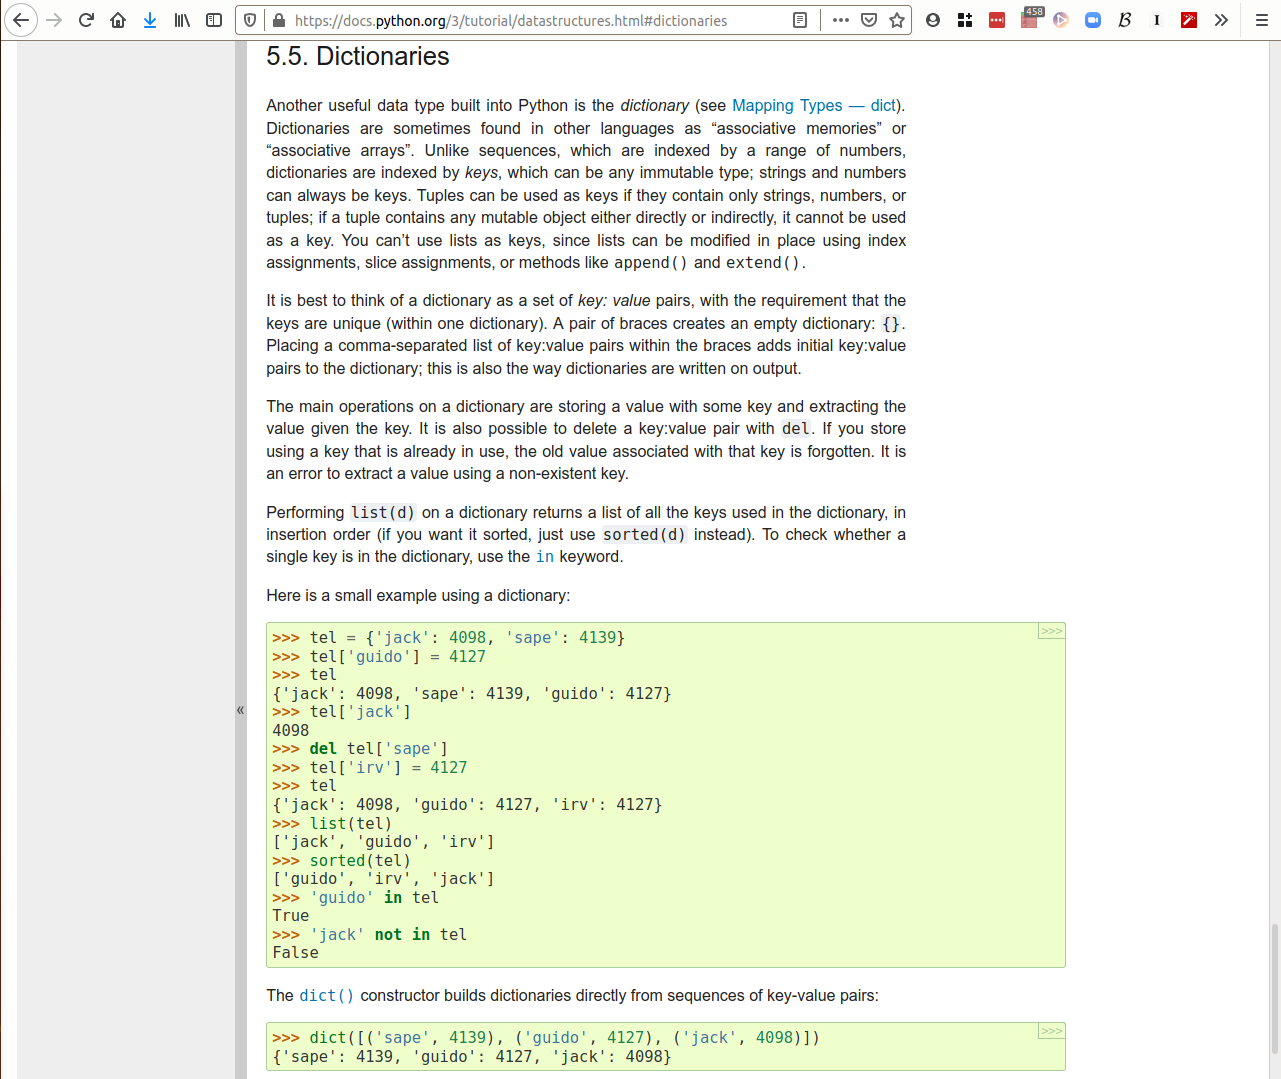
\includegraphics[width=\columnwidth]{figs/docs-dicts.png}
\end{frame}

\begin{frame}[fragile]
  \begin{example}[phone-small.py]
    \inputminted{python}{examples/phone-small.py}
  \end{example}
\end{frame}

\subsection{Sökning}

\begin{frame}[fragile]
  \mintinline[fontsize=\huge]{python}|item in dict|
\end{frame}

\begin{frame}[fragile]
  \begin{example}[isin.py]
    \inputminted{python}{examples/isin.py}
  \end{example}
\end{frame}

\begin{frame}[fragile]
  \begin{example}[isin-alt.py]
    \inputminted{python}{examples/isin-alt.py}
  \end{example}
\end{frame}

\begin{frame}[fragile]
  \begin{exercise}[search.py]
    \begin{itemize}
      \item Skriv ett program som låter oss mata in ett antal namn med 
        tillhörande telefonnummer.
      \item Därefter får vi söka bland namnen.
    \end{itemize}
  \end{exercise}
\end{frame}


\section{Iterationer med for-slingor}

\subsection{For-slingan}

\begin{frame}[fragile]
  \begin{minted}[fontsize=\huge,numbers=none]{python}
for item in container:
  print(item)
  \end{minted}
\end{frame}

\begin{frame}[fragile]
  \begin{example}
    \begin{minted}{python}
for i in range(10):
  print(i)
    \end{minted}
  \end{example}

  \begin{example}
    \begin{minted}{python}
for person in ["adam", "bertil", "cesar"]:
    print(person)
    \end{minted}
  \end{example}

  \begin{example}
    \begin{minted}{python}
phone = {"adam": "070123456", "bertil": "072123456"}
for person in phone:
    print(person)
    \end{minted}
  \end{example}
\end{frame}

\begin{frame}[fragile]
  \begin{example}
    \begin{minted}{python}
phone = {"adam": "070123456", "bertil": "072123456"}
for person in phone:
    print(person)
    \end{minted}
  \end{example}

  \begin{example}
    \begin{minted}[highlightlines=2]{python}
phone = {"adam": "070123456", "bertil": "072123456"}
for person, number in phone.items():
    print(f"{person} har telefonnummer {number}")
    \end{minted}
  \end{example}
\end{frame}

